\documentclass[11pt,a4paper]{article}
\usepackage{graphicx}
\usepackage{subfigure}
\usepackage{amsmath}
\usepackage{makecell}
\usepackage[utf8]{inputenc}
\usepackage{listings} %放代码
\usepackage{xcolor} %代码着色宏包
\usepackage{color}
\usepackage{xeCJK}
\usepackage{float}

%好像是数学的包
\usepackage{amsmath}
\usepackage{amssymb}
\usepackage{mathrsfs}
%页面布局包
\usepackage{geometry}
%画图包
\usepackage{tikz}
%画图背景包
\usetikzlibrary{backgrounds}

\geometry{left=3.0cm, right=3.0cm, top=3cm, bottom=3cm}

%自定义命令
\newcommand{\psiG}{\psi_{G}}
%在tikz中画一个顶点
%#1:node名称
%#2:位置
%#3:标签
\newcommand{\newVertex}[3]{\node[circle, draw=black, line width=1pt, scale=0.8] (#1) at #2{#3}}
%在tikz中画一条边
\newcommand{\newEdge}[2]{\draw [black,very thick](#1)--(#2)}
%在tikz中放一个标签
%#1:名称
%#2:位置
%#3:标签内容
\newcommand{\newLabel}[3]{\node[line width=1pt] (#1) at #2{#3}}


\title{Introduction to Computing Systems\\Homework 2}
\author{PB18111697 王章瀚}

\begin{document}
	\maketitle
	\section{}
	\subsection*{a}
	\begin{figure}[H]
		\centering
		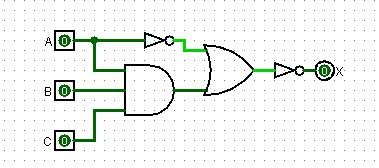
\includegraphics[width=1\linewidth]{1_a.jpg}
		\label{1_a}
	\end{figure}

	\subsection*{b}
	\begin{figure}[H]
		\centering
		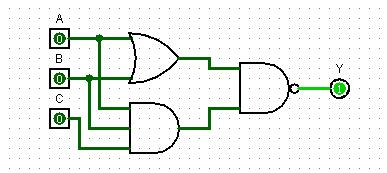
\includegraphics[width=1\linewidth]{1_b.jpg}
		\label{1_b}
	\end{figure}

	
	\section{}
	\subsection*{a}
	\subsubsection*{Way 1}
	As shown below, it needs 22 transistors in all.
	\begin{figure}[H]
		\centering
		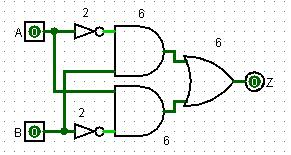
\includegraphics[width=1\linewidth]{2_a_1.jpg}
		\label{2_a_1}
	\end{figure}
	\subsubsection*{Way 2}
	As shown below, it needs 24 transistors in all.
	\begin{figure}[H]
	\centering
	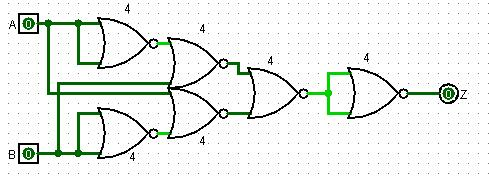
\includegraphics[width=1\linewidth]{2_a_2.jpg}
	\label{2_a_2}
	\end{figure}


	\subsection*{b}
	Below is the circuit.
	\begin{figure}[H]
		\centering
		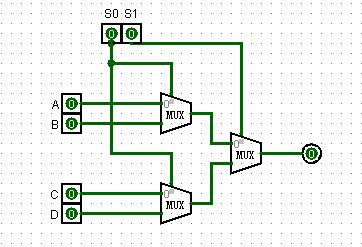
\includegraphics[width=1\linewidth]{2_b.jpg}
		\label{2_b}
	\end{figure}
	
	Below is the truth table.\par
	\begin{tabular}{|c|c|c|}
		\hline 
		S1 & S0 & OUT \\ 
		\hline 
		0 & 0 & A \\ 
		\hline 
		0 & 1 & B \\ 
		\hline 
		1 & 0 & C \\ 
		\hline 
		1 & 1 & D \\ 
		\hline 
	\end{tabular} 
	
	\section{}	
	\begin{figure}[H]
		\centering
		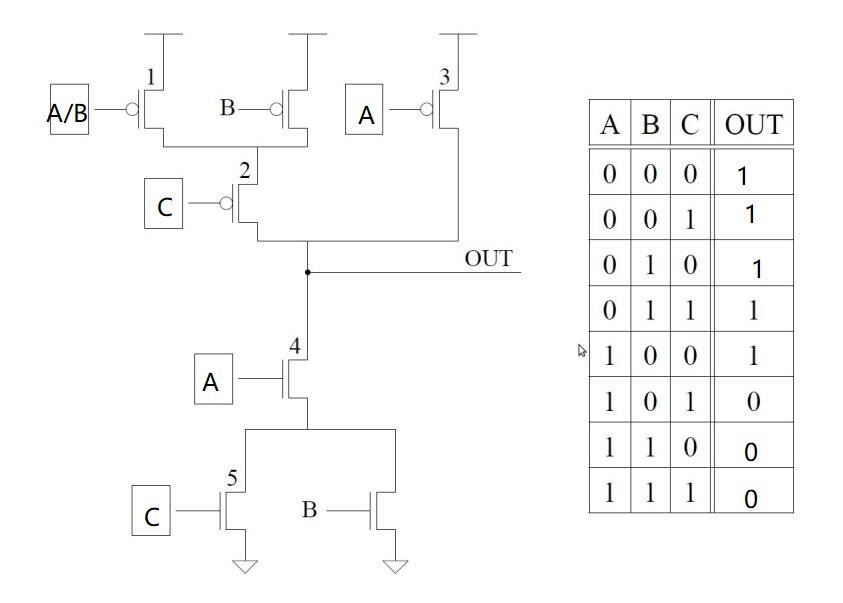
\includegraphics[width=1\linewidth]{3.jpg}
		\label{3}
	\end{figure}

	
	\section{3.19}
	When the input A goes from 0 to 1, output D in Figure 3.36 turns from the value of C to the value of D, while output D in Figure 3.37 will maintain its value. Besides, Figure 3.36 shows a combinational logic circuit while Figure 3.37 shows a sequential logic circuit.
	
	\section{Adapted from 3.25}
	a. 3\\
	b. 16\qquad \textcolor{red}{每个全加器3个延迟,总共3*4=12个}\\
	c. As shown below,
	\begin{figure}[H]
		\centering
		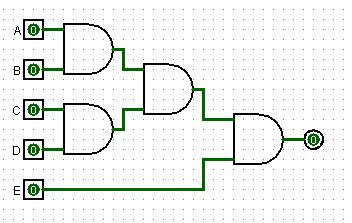
\includegraphics[width=1\linewidth]{5_c.jpg}
		\label{5_c}
	\end{figure}
	
	\section{3.26}
	As shown below,
	\begin{figure}[H]
		\centering
		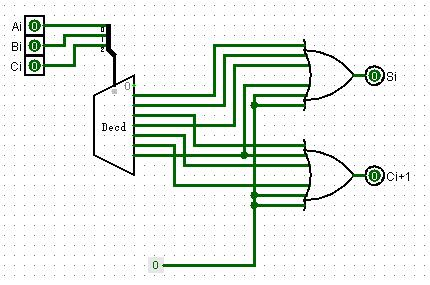
\includegraphics[width=1\linewidth]{6.jpg}
		\label{6}
	\end{figure}

	\section{}
	As shown below,
	\begin{figure}[H]
		\centering
		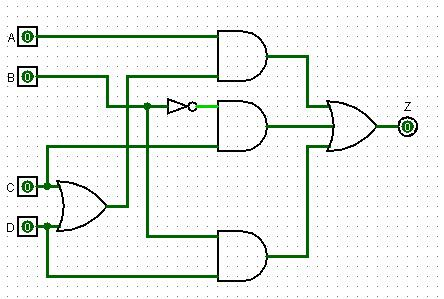
\includegraphics[width=1\linewidth]{7.jpg}
		\label{7}
	\end{figure}
	
	\section{Adapted from 3.30}
	\subsection*{a.}
	As shown below,\par
	\begin{tabular}{cc|ccc}
		\hline 
		A & B & G & E & L \\ 
		\hline 
		0 & 0 & 0 & 1 & 0 \\ 
		\hline 
		0 & 1 & 0 & 0 & 1 \\ 
		\hline 
		1 & 0 & 1 & 0 & 0 \\ 
		\hline 
		1 & 1 & 0 & 1 & 0 \\ 
		\hline 
	\end{tabular} 
	\subsection*{b.}
	As shown below,\par
	\begin{figure}[H]
		\centering
		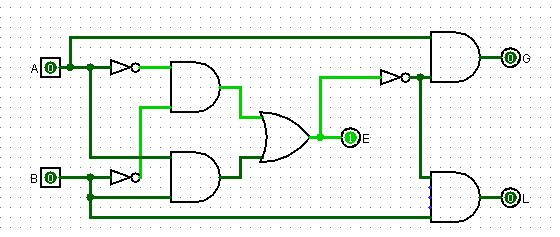
\includegraphics[width=1\linewidth]{8_b.jpg}
		\label{8_b}
	\end{figure}

	\subsection*{c.}
	As shown below,\par
	\begin{figure}[H]
	\centering
	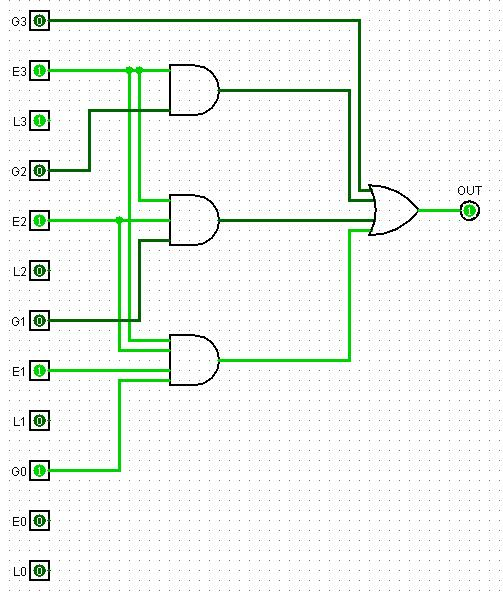
\includegraphics[width=1\linewidth]{8_c.jpg}
	\label{8_c}
	\end{figure}
	
	
	\section{}
	\textcolor{red}{
		正确的顺序应该是这样的:000000, \underline{100000, 111000, 111110, 011111, 000111, 000001}, 100000...周期是6,所以50个周期以后,是111000
	}\par
	After the first cycle, the state becomes 100000, due to the input of the first D Letch is 1. After the second cycle, it turns into 110000. And then 111000, 111100, 111110, 111111, 011111, 001111, 000111, 000011, 000001, 000000. Here are 12 states in total.\par
	As we can see, after 50 cycles, the state will be changed to \underline{110000}. And it takes \underline{12} cycles for a specific state to show up again.
	
	
	
	\section{}
	\subsection*{a.}
	\textcolor{red}{
		应该是(100*100)*4*100*4*101*2*901 = 2912032000000
	}\par
	The number of the whole states is $100+100+4+100+4+50+50+2+60*15=1310$. So the minimum number of bits that we need to use to store the state required is $\lceil log_{2}1310 \rceil = \underline{11}$.
	\subsection*{b.}
	(1). 
		\textcolor{red}{
			应该是7*2bits
		}\par
		 $\lceil log_{2}(100+100) \rceil = \underline{8}$\\
	(2). $\lceil log_{2}4 \rceil = \underline{2}$\\
	(3). $\lceil log_{2}100 \rceil = \underline{7}$\\
	(4). $\lceil log_{2}4 \rceil = \underline{2}$\\
	(5). $\lceil log_{2}(50+50) \rceil = \underline{7}$\\
	(6). $\lceil log_{2}2 \rceil = \underline{1}$\\
	(7). $\lceil log_{2}(15*60) \rceil = \underline{10}$\\
	\subsection*{c.}
	First, since these variables are not quite relevant, so they can just be seperated to build several simpler circuits instead of a complex circuit.
	Second, the gates number that a circuit used to decode a 11 bits data will be larger than that for serveral data with 8,2,7,2,7,1,10 bits.


	\section{}
	\subsection*{a.}
	The truth table is shown below.\par
	\begin{tabular}{cccc|cc}
		\hline 
		floor[1] & floor[0] & $Q^{n}[1]$ & $Q^{n}[0]$ & $Q^{n+1}[1]$ & $Q^{n+1}[0]$ \\ 
		\hline 
		0 & 0 & 0 & 0 & 0 & 0 \\ 
		\hline 
		0 & 0 & 0 & 1 & 0 & 1 \\ 
		\hline 
		0 & 0 & 1 & 0 & 0 & 0 \\ 
		\hline 
		0 & 0 & 1 & 1 & 0 & 0 \\ 
		\hline 
		0 & 1 & 0 & 0 & 0 & 0 \\ 
		\hline 
		0 & 1 & 0 & 1 & 0 & 1 \\ 
		\hline 
		0 & 1 & 1 & 0 & 1 & 0 \\ 
		\hline 
		0 & 1 & 1 & 1 & 0 & 1 \\ 
		\hline 
		1 & 0 & 0 & 0 & 1 & 0 \\ 
		\hline 
		1 & 0 & 0 & 1 & 0 & 1 \\ 
		\hline 
		1 & 0 & 1 & 0 & 1 & 0 \\ 
		\hline 
		1 & 0 & 1 & 1 & 1 & 1 \\ 
		\hline 
		1 & 1 & 0 & 0 & 1 & 1 \\ 
		\hline 
		1 & 1 & 0 & 1 & 1 & 1 \\ 
		\hline 
		1 & 1 & 1 & 0 & 1 & 0 \\ 
		\hline 
		1 & 1 & 1 & 1 & 1 & 1 \\ 
		\hline 
	\end{tabular} 
	\subsection*{b.}
	\begin{figure}[H]
		\centering
		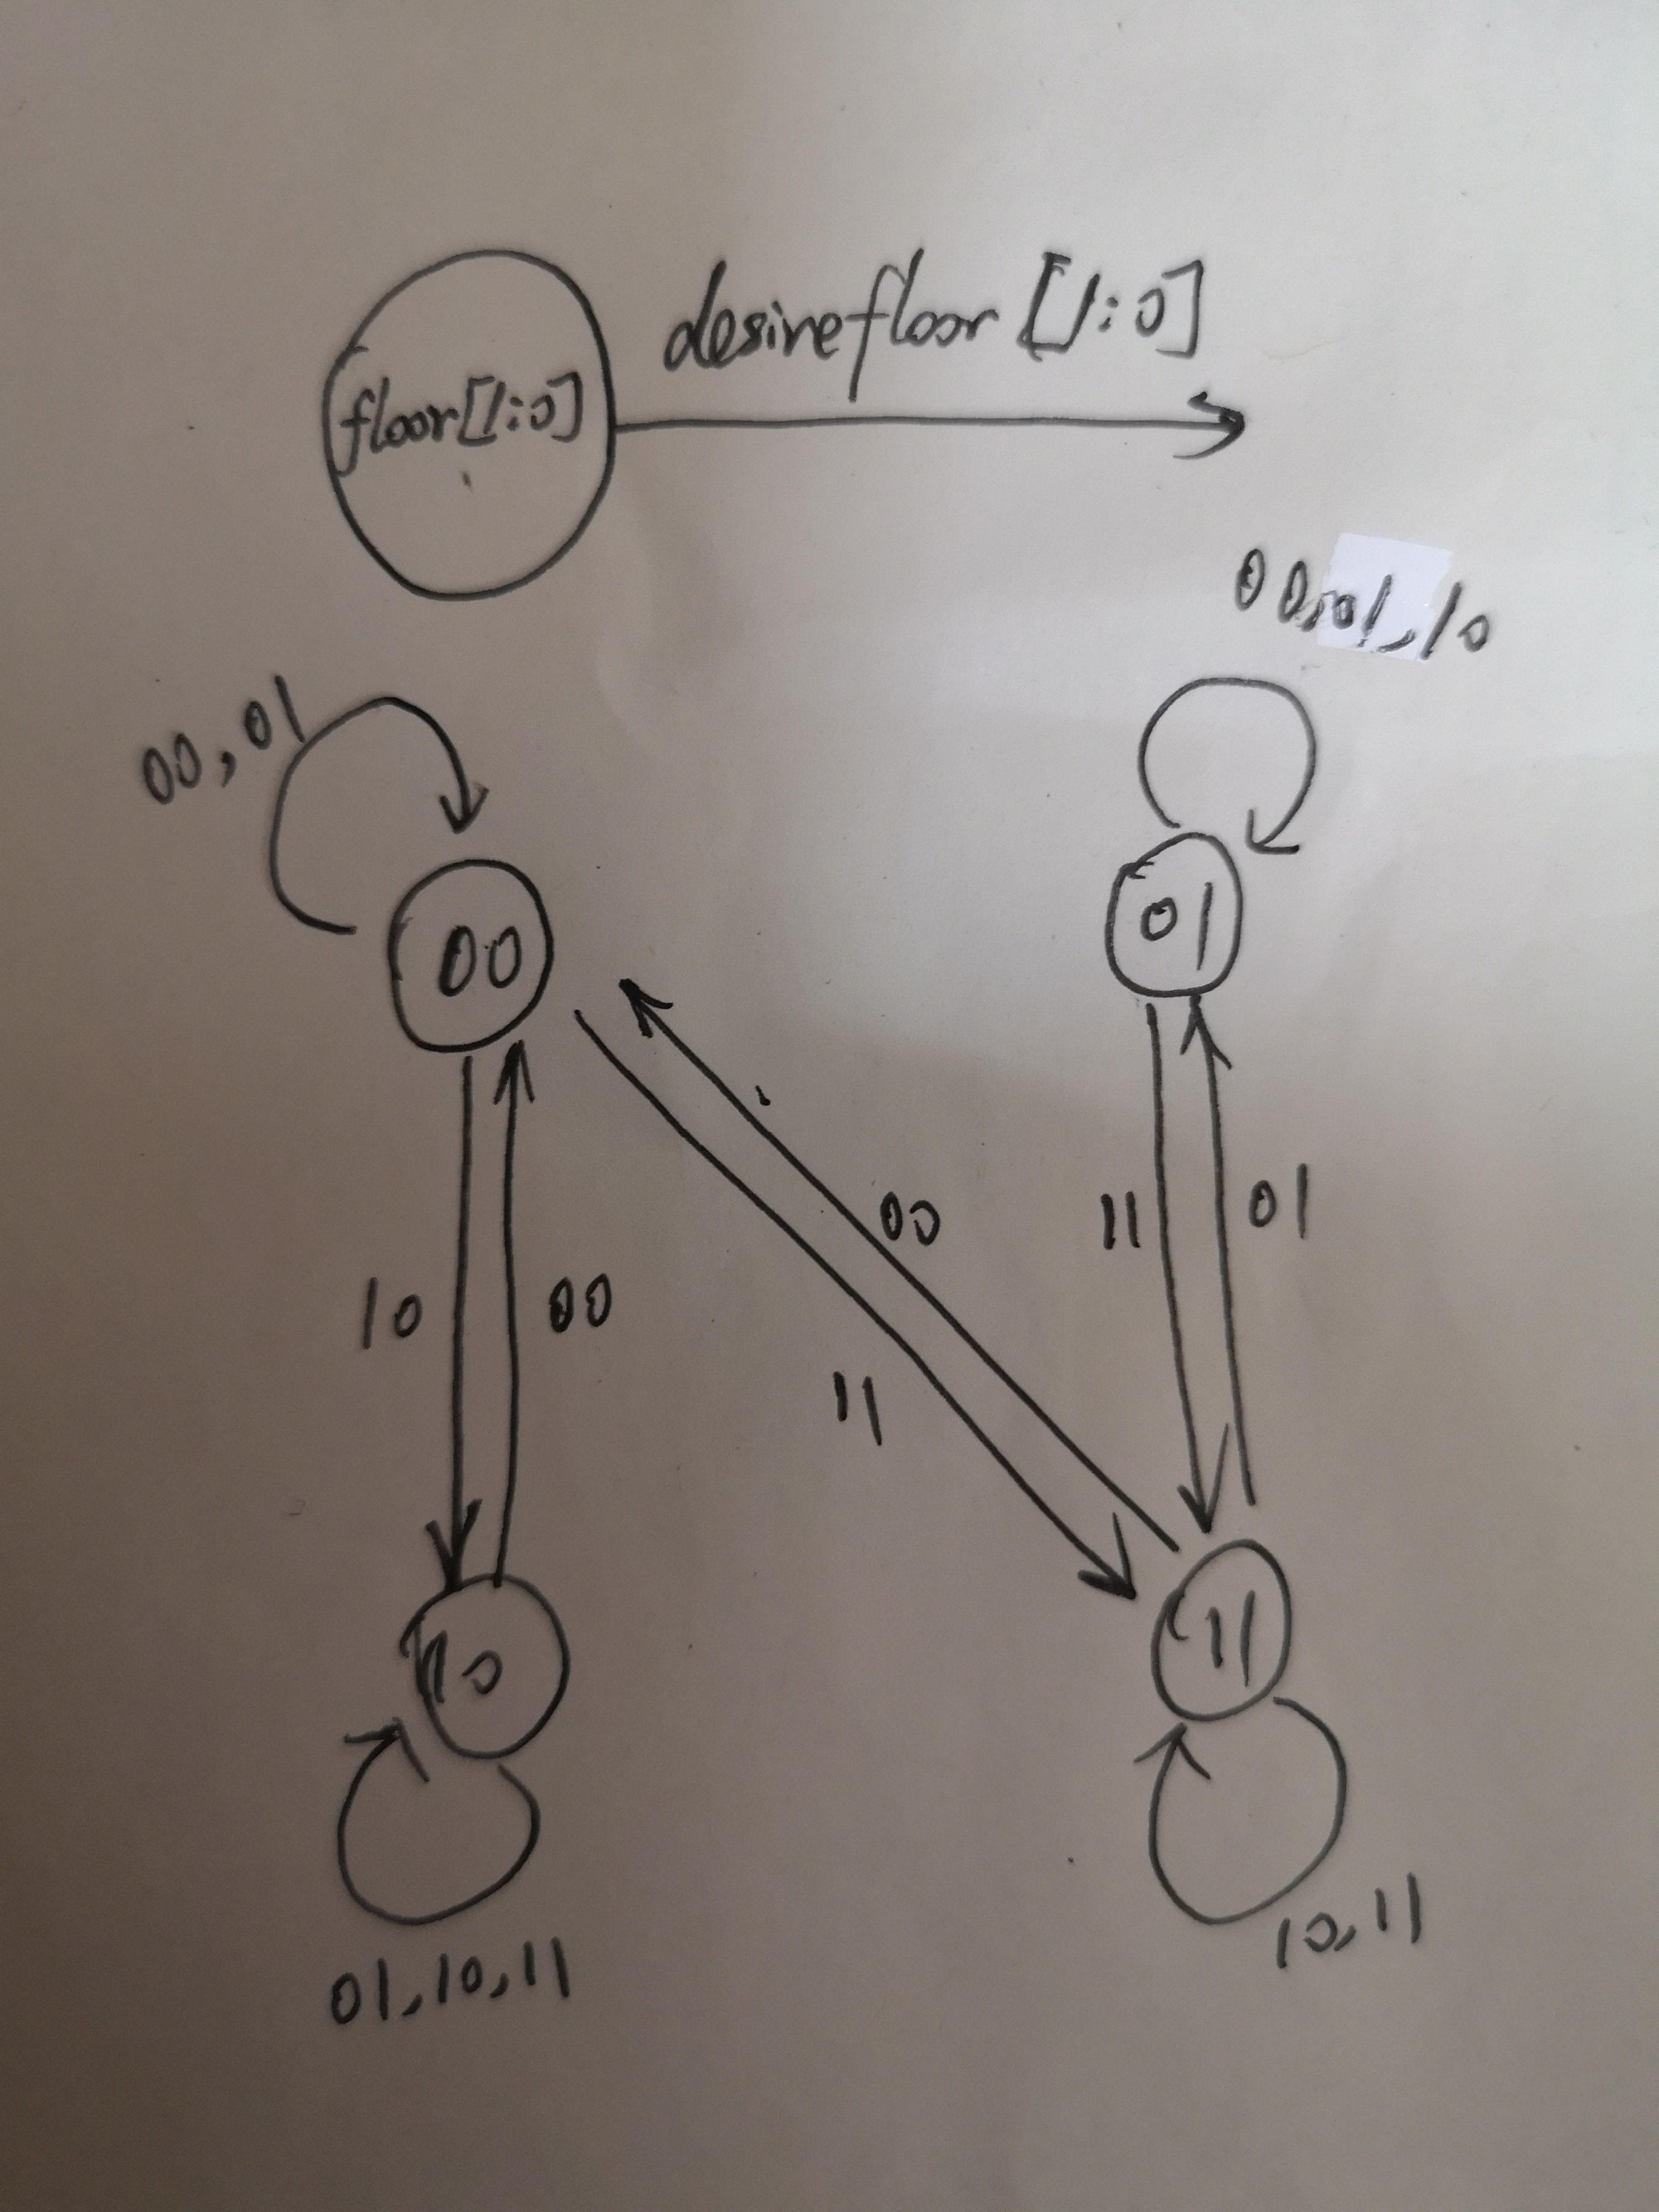
\includegraphics[width=1\linewidth]{11_b.jpg}
		\label{11_b}
	\end{figure}
	
	
	

	
\end{document}